\documentclass[10pt,a4paper]{article}
\usepackage[margin=0.82in]{geometry}
\usepackage{graphicx,booktabs,amsmath,amssymb,hyperref,microtype,array,caption}
\usepackage[T1]{fontenc}
\hypersetup{colorlinks=true,linkcolor=blue,citecolor=blue,urlcolor=blue}
\title{Evaluating Risk-Adaptive Checkpoints for Failure Containment in Chained Tool-Calling Agents: A Controlled Simulation Study}
\author{Ujjwal Gupta\\MDE2026004\\Indian Institute of Information Technology Allahabad}
\date{November 2026}
\begin{document}\maketitle
\begin{abstract}
Autonomous agents execute sequences of dependent tool calls, creating opportunities for faults to persist and influence consequential actions. Earlier research and review manuscripts identified a need for quantified comparisons of checkpoint placement and cascading failures. This paper reports a reproducible, synthetic fault-injection study comparing no checkpoints, fixed-interval post-action verification and risk-adaptive pre-action verification. We executed 18,000 primary chain-policy trials across lengths 6, 12 and 24, five deterministic seeds and 2,000 matched scenarios per length. Strict success requires both a clean final state and zero unsafe high-risk actions. At chain length 24, the no-checkpoint, fixed and adaptive policies achieved success rates of 15.00\%, 22.35\% and 24.70\%, respectively; adaptive verification lowered the fraction of runs with at least one unsafe action from 83.35\% (none) to 72.80\%, at the cost of 7.238 reviews per chain on average versus 6.000 for fixed checks. Sensitivity tests show adaptive performance declines with imperfect risk recognition. These results establish a transparent systems-level illustration of a safety--effort trade-off, not an estimate of real LLM-agent performance.
\end{abstract}
\noindent\textbf{Keywords:} tool-calling agents, failure propagation, risk-adaptive checkpoints, fault injection, system reliability, reproducibility
\section{Introduction}
Large language model (LLM) agents combine planning, tool invocation and observations over multiple actions. A flawed intermediate state can affect subsequent decisions, and a locally successful call need not satisfy the original goal. The supplied original research paper describes planning, state-tracking, error propagation and prompt-injection failures, and argues that verification should be considered at the level of whole tool chains \cite{gupta_original}. The associated review develops a taxonomy and identifies the lack of standardized failure benchmarks, limited causal analysis and uncertain placement of human checkpoints \cite{gupta_review}.

This work narrows that broad agenda to a measurable systems question: \emph{under controlled faults, how do no verification, periodic verification and risk-adaptive verification compare on chain success, unsafe action exposure and review burden?} The contribution is not a new LLM model and is not claimed to be a reproduction of published agent benchmark scores. Instead, it is a fully specified simulator intended to demonstrate what can and cannot be learned from different checkpoint policies.
\section{Literature Bridge and Research Gaps}
ReAct interleaves reasoning with observations \cite{react}, while realistic interactive benchmarks such as WebArena stress long-horizon behavior \cite{webarena}; AgentDojo addresses adversarial tool-content conditions \cite{agentdojo}. The supplied manuscripts synthesize these themes but do not provide an executed, controlled comparison between checkpoint schedules \cite{gupta_original,gupta_review}. Specifically, the review's sections on unclear checkpoint placement, error propagation, reproducible evaluation and human monitoring motivate three practical gaps: (i) insufficient chain-level metrics, (ii) unclear safety versus reviewer-cost trade-offs, and (iii) sensitivity to fallible risk identification. The current experiment addresses these gaps \emph{within a synthetic model only}. We do not establish novelty relative to the entire research literature, and bibliographic metadata for external works was carried over from the supplied paper rather than independently audited.
\section{Research Questions and Hypotheses}
\textbf{RQ1:} Do verification strategies improve strict end-to-end success relative to no checkpoints as chains lengthen? \textbf{RQ2:} Does risk-adaptive pre-action verification offer lower unsafe-action exposure than fixed-interval post-action checking, and at what review cost? \textbf{RQ3:} How sensitive is the adaptive policy to imperfect recognition of high-risk actions?

We expected review-based approaches to contain persistent faults more effectively than no checks. A stronger claim that adaptive verification is universally better than fixed checking was intentionally not assumed; this question depends on verification timing, fault distributions and reviewer burden.
\section{Methods}
\subsection{Synthetic environment and task state}
A workflow has $L\in\{6,12,24\}$ sequential tool actions. Each action is randomly designated high-risk with probability $0.30$ and low-risk otherwise. Exogenous fault probabilities are $0.17$ for high-risk and $0.035$ for low-risk actions. Each injected fault changes a Boolean internal state to \emph{corrupted}; in the absence of successful verification, corruption persists across later calls. A high-risk action executed while the state is corrupted counts as an unsafe action. No real private data or external action is involved. This deliberately simplified state machine captures persistence but not agent deliberation, privileges, prompt injection or real tool semantics.

A verification step detects and repairs a corrupted state with probability $0.92$; a clean state remains clean. Exogenous fault draws and risk labels are shared among policies within each trial. Detection outcomes use predetermined random draws so the same candidate checkpoint is reproducible. The single state variable is an abstraction rather than a faithful model of a particular LLM.
\subsection{Policies and algorithm}
\textbf{None:} execute all steps without review. \textbf{Fixed:} verify after steps 4, 8, 12 and so forth. \textbf{Adaptive:} verify immediately \emph{before} an identified high-risk step. The latter attempts to remove earlier contamination before a consequential operation; however, it cannot prevent a fresh fault caused by that very action. This distinction is important: the comparison examines two \emph{checkpoint-placement policies}, not identical timing with only different schedules.

At step $i$, let $C_i$ indicate the corrupted state after any policy-specific pre-check, and let $E_i\sim\mathrm{Bernoulli}(p_i)$ be a new fault. After execution, $C'_i=C_i\lor E_i$. If action $i$ is high-risk and $C'_i=1$, unsafe-action count increments. A successful verification maps $C'=1$ to $C=0$ for the next step. Recovered state does not erase an unsafe action already recorded. This prevents a terminal state repair from being mistaken for complete task success.
\subsection{Experimental protocol and metrics}
Five fixed seeds (11, 29, 47, 83, 101) generated 400 scenarios for each length, producing 2,000 paired scenarios per length. Every scenario was evaluated under all three policies: $3\times 3\times 2{,}000=18{,}000$ primary runs. The primary metric is strict task success: final state clean \emph{and} no unsafe high-risk action anywhere in the chain. Secondary metrics are the proportion of runs containing any unsafe action, mean count of unsafe actions, human reviews per chain, recovery events and clean terminal-state rate. A sensitivity experiment repeats scenarios with high-risk recognition recalls of 0.50, 0.75 and 1.00, while keeping fault probabilities fixed. No real participant or human reviewer was recruited; a probabilistic detection process models hypothetical review effectiveness.

All code, seed values and parameters are preserved in \texttt{configs/protocol.json}; per-trial records are saved in \texttt{results/trial\_results.csv}. This is an analytic evaluation of a simulated process; there are no training or test splits, no learned parameters and no risk of label leakage from a training phase.
\section{Results}
\begin{table}[ht]\centering\caption{Measured primary results. Each policy/length cell contains 2,000 trials. Success and unsafe-run metrics are percentages; reviews are counts per chain.}\label{tab:primary}
\small\begin{tabular}{rrrrr}\toprule
$L$ & Policy & Success (\%) & Unsafe runs (\%) & Reviews\\\midrule
6 & None & 63.45 & 29.90 & 0.000\\
6 & Fixed & 68.50 & 27.85 & 1.000\\
6 & Adaptive & 68.95 & 24.30 & 1.776\\
12 & None & 40.15 & 55.55 & 0.000\\
12 & Fixed & 48.80 & 50.70 & 3.000\\
12 & Adaptive & 48.95 & 45.95 & 3.641\\
24 & None & 15.00 & 83.35 & 0.000\\
24 & Fixed & 22.35 & 77.65 & 6.000\\
24 & Adaptive & 24.70 & 72.80 & 7.238\\\bottomrule
\end{tabular}\end{table}

\begin{figure}[ht]\centering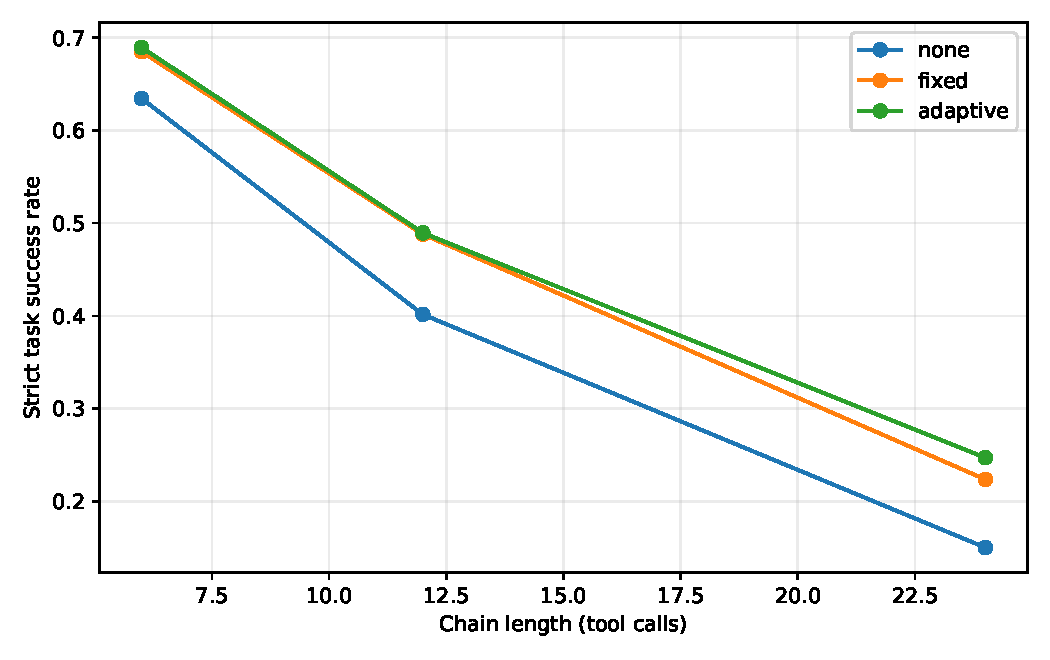
\includegraphics[width=.82\linewidth]{figures/success_by_length.pdf}\caption{Strict chain success decreases with length under all policies. Values are direct aggregates of actual simulator runs.}\label{fig:success}\end{figure}

At $L=24$, risk-adaptive success exceeds fixed checking by 2.35 percentage points and no checkpoints by 9.70 percentage points. For shorter chains, the success difference between adaptive and fixed is small (0.45 and 0.15 points). These are descriptive results; no statistical significance or real-world causal effect is asserted.

\begin{figure}[ht]\centering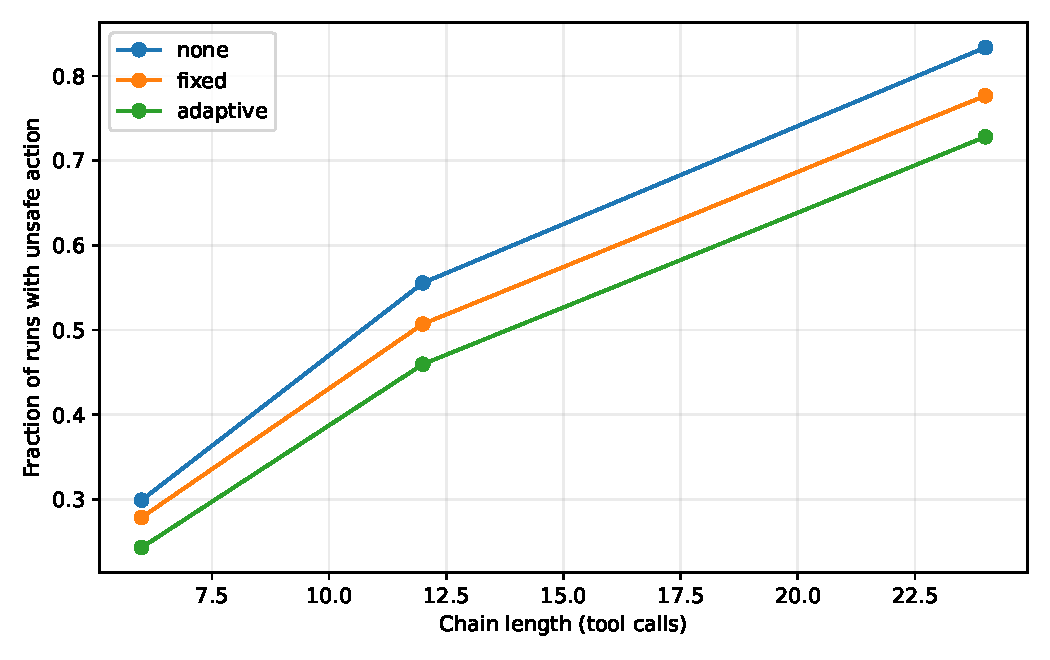
\includegraphics[width=.82\linewidth]{figures/unsafe_by_length.pdf}\caption{Observed fraction of simulated workflows with at least one unsafe action. Lower is better.}\label{fig:unsafe}\end{figure}

Adaptive checking has the lowest rate of unsafe-run exposure at all tested lengths. At $L=24$ it reduces the mean count of unsafe actions from 4.3875 (none) to 1.3180; fixed checking yields 1.9950. Nevertheless, every policy exhibits considerable unsafe exposure in long chains because faults can arise during an already-running high-risk action.

\begin{figure}[ht]\centering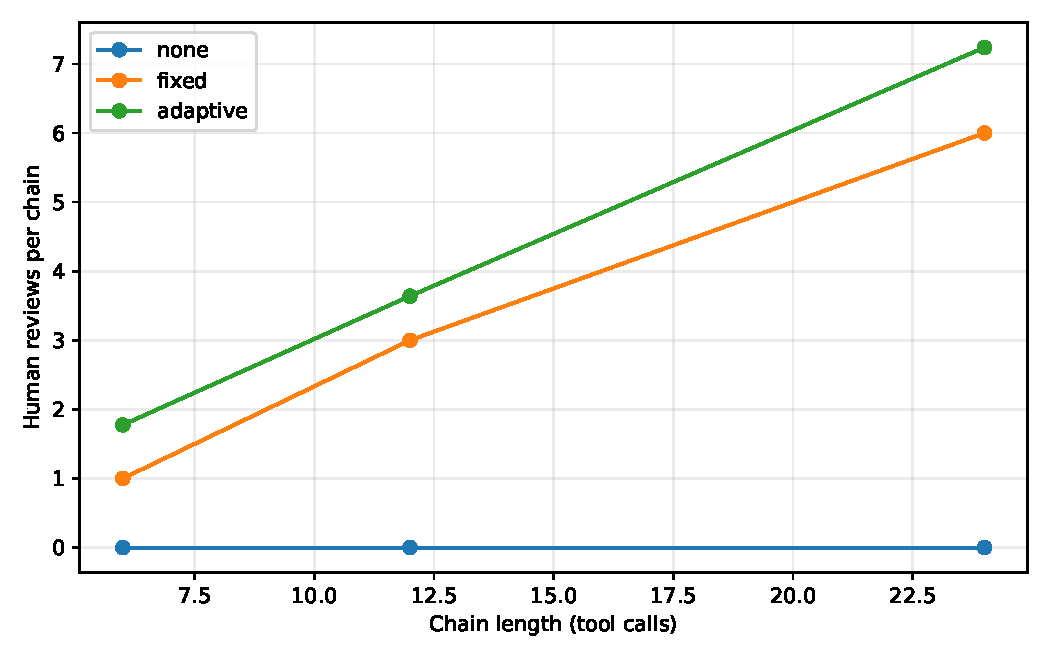
\includegraphics[width=.82\linewidth]{figures/review_cost.pdf}\caption{Mean review burden increases with chain length. Adaptive verification checks high-risk actions and is not review-free.}\label{fig:reviews}\end{figure}

\subsection{Sensitivity to imperfect risk recognition}
\begin{table}[ht]\centering\caption{Sensitivity of adaptive checking to high-risk recognition recall, at chain length 24 (2,000 trials per setting).}\small
\begin{tabular}{rrrr}\toprule Recall & Success (\%) & Unsafe runs (\%) & Reviews\\\midrule
0.50 & 20.00 & 77.95 & 3.613\\
0.75 & 22.20 & 75.45 & 5.458\\
1.00 & 24.70 & 72.80 & 7.238\\\bottomrule
\end{tabular}\end{table}
\begin{figure}[ht]\centering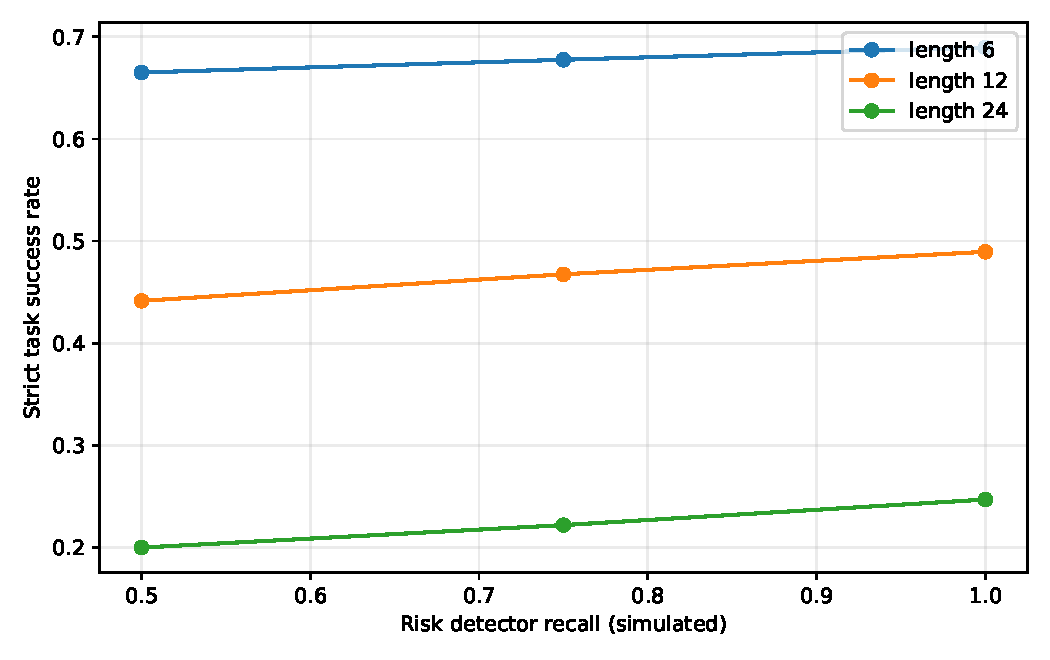
\includegraphics[width=.82\linewidth]{figures/risk_sensitivity.pdf}\caption{Sensitivity curves across all three chain lengths. Review gains depend on identifying hazardous transitions.}\label{fig:sensitivity}\end{figure}

Reducing risk recognition recall from 1.00 to 0.50 decreases success at $L=24$ by 4.70 percentage points. The change also reduces the review burden from 7.238 to 3.613 checks per chain, making the safety--effort tension explicit.
\section{Discussion}
The experiment supports a qualified proposition: verification can limit the persistence of corruption and reduce unsafe downstream actions. It does not show that adaptive checkpoints guarantee safety or are always more efficient. Under the selected probability model, adaptive checks consume more reviewer effort than the fixed schedule, and at $L=6$ and $L=12$ strict-success gains over fixed checking are minimal. Adaptive checks reduce unsafe exposures more consistently than they improve terminal-state cleanliness; fixed checks produce higher clean-end rates because they often check at the final step. This discrepancy illustrates why a clean final state is an inadequate proxy for safety over the full chain.

The mechanism is interpretable: pre-action checking can cleanse inherited corruption before a high-risk operation, whereas a post-action review may detect corruption only after the unsafe act has occurred. However, the timing asymmetry is a potential confound. A more comprehensive follow-up should compare adaptive and fixed policies at matched review budgets and matched pre-action timing, vary detector specificity and measure false positives.
\section{Threats to Validity and Limitations}
\textbf{Construct validity:} a single Boolean corruption state cannot capture changing beliefs, model reasoning, tool-output ambiguity, permission boundaries or prompt injection. Risk labels are synthetic and treated as knowable; real systems must infer risk. Detection effectiveness and fault probabilities are chosen experimental assumptions rather than empirically calibrated estimates.
\textbf{Internal validity:} paired scenarios hold fault draws and risk distributions constant. However, checkpoint timing differs by design, so improvements cannot be attributed solely to risk-based scheduling. Detector noise is shared only through deterministic scenario draws; future studies should examine independent reviewer errors and cost models.
\textbf{External validity:} no live LLM, official agent benchmark, real API or human subjects were evaluated. Results cannot predict deployment incident rates, establish safety guarantees, or independently verify the published benchmark statistics discussed by the source papers.
\textbf{Statistical scope:} the reported quantities are descriptive sample means from a synthetic simulator. Seeds reflect stochastic scenario variability, not independent real-world deployments. No hypothesis-test p-values are claimed.
\section{Conclusion and Future Work}
A reproducible simulated tool-chain study found that risk-adaptive pre-action verification reduced unsafe-action exposure relative to both no checking and periodic post-action verification, while consuming additional review effort. Strict success remained low for 24-step workflows, and adaptive benefits declined with imperfect risk recognition. The central lesson is not that a particular checkpoint strategy is universally superior, but that safety requires chain-level measurement, explicit accounting for irreversible actions and careful treatment of the reviewer cost. Future work should evaluate matched-budget policies, model realistic false alarms and rollback, and test agent-generated traces in real tool environments before translating these trends into operational claims.
\section*{Reproducibility and AI use}
The source code, configurations, full per-trial CSV files, plotting scripts, basic sanity tests and actual execution log accompany the submission. An AI assistant assisted with experimental design, code construction, execution and drafting. Parameter assumptions, manuscript claims and executable evidence must be inspected and defended by the student; no real LLM experiment is claimed.
\begin{thebibliography}{9}
\bibitem{gupta_original} U. Gupta, ``Failure Modes in Chained Tool-Calling Agents Operating Without Human Checkpoints,'' original course research manuscript, 2026.
\bibitem{gupta_review} U. Gupta, ``Failure Modes in Chained Tool-Calling Agents Operating Without Human Checkpoints,'' course review manuscript, 2026.
\bibitem{react} S. Yao et al., ``ReAct: Synergizing Reasoning and Acting in Language Models,'' ICLR, 2023.
\bibitem{webarena} S. Zhou et al., ``WebArena: A Realistic Web Environment for Building Autonomous Agents,'' ICLR, 2024.
\bibitem{agentdojo} E. Debenedetti et al., ``AgentDojo: A Dynamic Environment to Evaluate Prompt Injection Attacks and Defenses for LLM Agents,'' NeurIPS, 2024.
\end{thebibliography}
\end{document}
